\documentclass[12pt, a4paper, titlepage, onehalfspacing]{report}
\usepackage[utf8]{inputenc} % Characters, including Hungarian letters
\usepackage[sorting=none]{biblatex} % Imports biblatex package
\addbibresource{sample.bib} % Import the bibliography file
\usepackage[T1]{fontenc} % Output font encoding for international characters
\usepackage[unicode]{hyperref}
\usepackage[english]{babel}
\usepackage[left=2.50cm, right=2.50cm, top=2.50cm, bottom=2.50cm]{geometry}\usepackage{graphicx}
\usepackage{comment}
\usepackage{setspace}
\graphicspath{ {images/} }
\usepackage[section]{placeins}
\usepackage{float}
\usepackage{multirow}
\usepackage{tabularx}
\usepackage{algorithm} 
\usepackage{algpseudocode}
\usepackage{titlesec}
\usepackage{amssymb}
\usepackage{amsmath}
\usepackage{multirow}
\usepackage{csquotes}
\usepackage{gensymb}
\usepackage{booktabs}
\usepackage{subcaption}

\titleformat{\chapter}[display]
{\normalfont\huge\bfseries}{\chaptertitlename\ \thechapter}{20pt}{\Huge}

\date{\today}

\begin{document}
\begin{titlepage}
\begin{center}

{ \LARGE \textbf{Master's Thesis}\\[2.5cm]}
{ \LARGE \textbf{Vehicle Speed Estimation Based on Artificial Intelligence Algorithms}\\ [2.5cm]}
{\normalsize \emph{Author:}}\\
{ \large \bfseries Andrzej Skrodzki}\\[4cm]


\includegraphics[width=70mm]{images/BMElogo.png}\\[0.5cm]
{\normalsize Budapest University of Technology and Economics\\ Department of Control for Transportation and Vehicle Systems\\[2.5cm]}

\begin{minipage}{0.7\textwidth}
\centering
{\normalsize \emph{Supervisor:} \\
 \bfseries Donát Rácz}\\
\end{minipage}

\vfill
{\normalsize  Master's Thesis, \\\large \today}\\[0.5cm]

\end{center}
\end{titlepage}   
\newpage
\pagenumbering{roman}

%% Extra page for marking sources, for example:
%\begin{center}
%{\vspace{5cm}\large \bfseries EFOP-3.6.3-VEKOP-16-2017-00001:}\vspace{5cm}\\

\tableofcontents

%ezt ki kell majd tölteni!!!
%\begin{abstract}
%This is the place for any abstract...
%\end{abstract}

\include{Chapters/1_introduction}

\include{Chapters/2_development_environment}

\include{Chapters/3_direct_estimation}

\chapter{AI aided conventional estimation}

In the previous chapter the direct estimation of vehicle speeds with different AI models was discussed. In this chapter the focus will be shifted towards combining conventional estimation methods with AI algorithms to improve the overall performance of the estimator. First a simple wheel speed based vehicle speed estimation method will be presented. Then a model based estimator will be discussed that utilizes the linear tire model to estimate the vehicle speed from the tire forces. Furthermore an Extended Kalman Filter (EKF) based estimator will be developed that fuses the previously derived model based estimator as the state transition function and the wheel speed based estimator as the measurement function. Finally, the best performing AI models from the previous chapter will be combined with the EKF based estimator to improve its performance.

\section{Simple wheel speed based estimation}

\section{Model based estimation using linear tire model}

\section{Extended Kalman Filter based estimation}

\subsection{Conventional EKF}

\subsection{AI aided EKF}

\chapter{Real Time Impelementation}

In this chapter the real time implementation of the trained networks will be described. The main focus will be on integrating the model into an environment where it can process the incoming data in real time and provide estimations with as little latency as possible. 

\section{Development Environment}

Before describing the development environment, the meaning behind real time implementation should be clarified. In this context, real time means that the model is able to process incoming data and provide estimations within a fixed time frame, which is determined by the system. Within every defined time step, the computational unit (eg. microcontroller) receives new input data at the beginning of the time step, processes it using the implemented model, and outputs the estimation before the next time step begins. This setup can be seen on figure \ref{fig:rt}

\FloatBarrier
\begin{figure}[h]
    \centering
    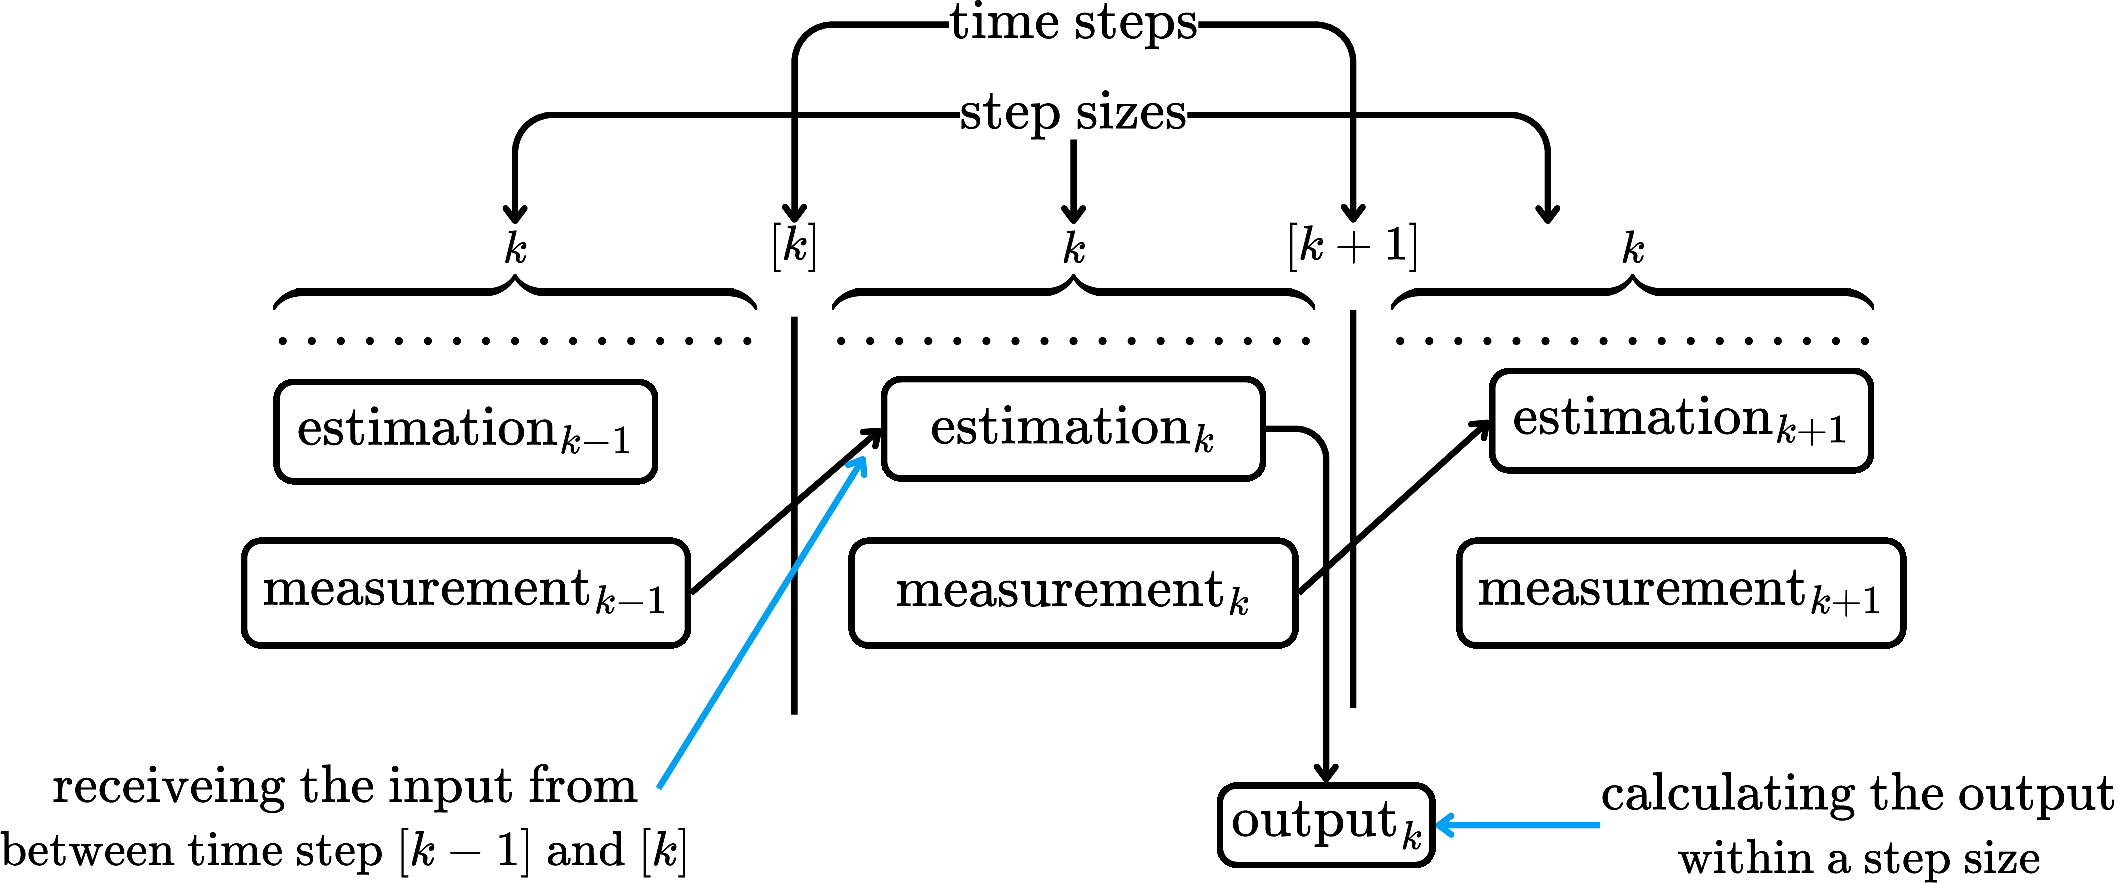
\includegraphics[width=0.9\textwidth]{images/rt.pdf}
    \caption{Real time implementation concept}
    \label{fig:rt}
\end{figure}
\FloatBarrier

A possible development environment for implementing an arbitrary control or estimation algorithm for vehicle application can be a toolchain offered by dSpace. This toolchain allows the user to create models in MATLAB Simulink, generate C code from these models and utilize the generated code on the hardware developed by dSace, where it can be tested in real time. The hardware can be connected to a real vehicle via the CAN bus, or to a simulator for cost efficiency reasons. In this thesis the latter application was chosen, using the BeamNG.drive simulator. The main steps of the real time implementations are the following:
\begin{enumerate}
    \item Prepare the trained models in MATLAB using the Deep Learning Toolbox (DLT).
    \item Integrate the trained models into MATLAB Simulink using DLT.
    \item Generating C code from the Simulink model using dSpace's ConfigurationDesk software.
    \item Deploying the generated code on dSpace's MicroAutoBox hardware using ControlDesk software.
    \item Connecting the MicroAutoBox to computer that runs BeamNG.drive via CAN bus.
    \item Testing the real time performance of the models with different step sizes.
\end{enumerate}
The toolchain of the real time implementation is illustrated in Figure \ref{fig:rt_toolchain}.
\FloatBarrier
\begin{figure}[h]
    \centering
    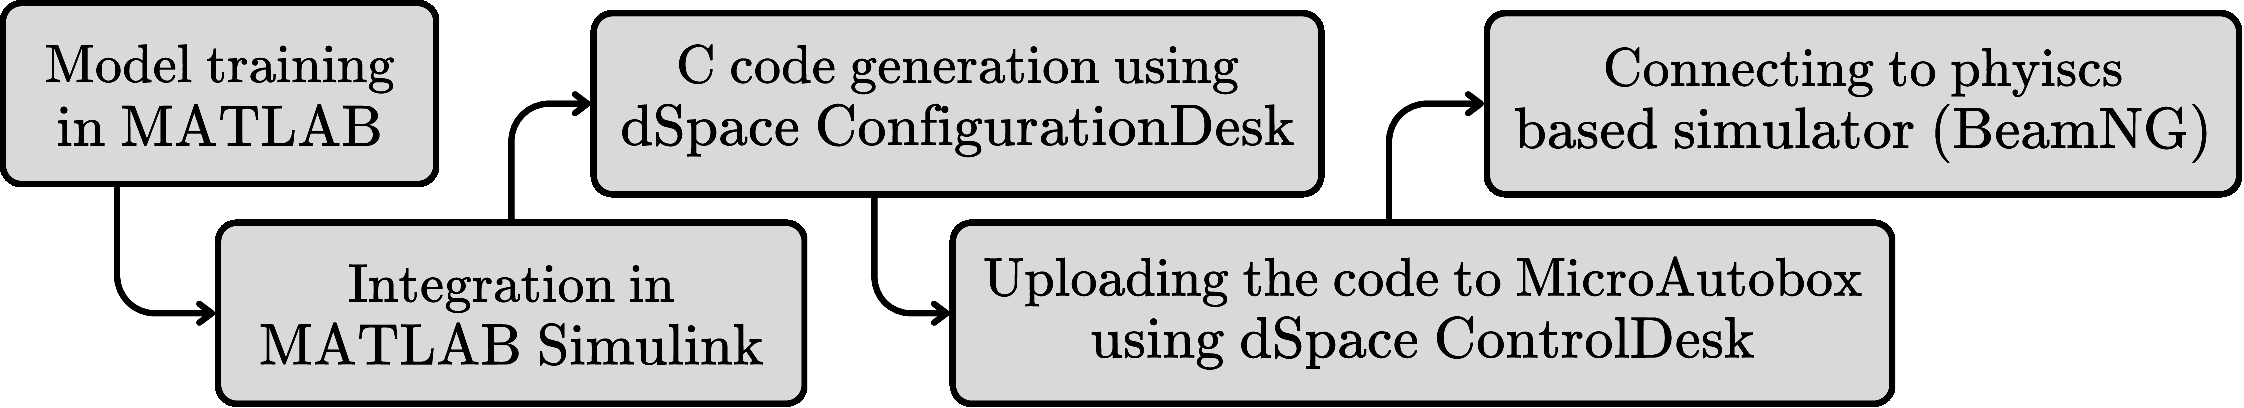
\includegraphics[width=0.9\textwidth]{images/rt_toolchain.pdf}
    \caption{Toolchain of the real time implementation}
    \label{fig:rt_toolchain}
\end{figure}
\FloatBarrier
The main question to answer is what is the smallest step size that the MicroAutoBox requires to be able to run the model. In other words, how much time does the MicroAutoBox need to process the inserted model and provide and estimation. This is crucial question since the smaller the step size, the more accurate and responsive the estimation will be, which can result better overall performance in a control application. 

\section{Results}

The chosen models for real time implementation were the best performing LSTM, GRU and the TCN architectures described in Chapter \ref{ch:direct_estimation}. Before starting the tests, a short calculation was made to estimate the FLOPS (floating point operations per second) required by each model. This gives a rough idea about the computational requirements of the models, which can be compared to the capabilities of the MicroAutoBox hardware. The calculated FLOPS are the following:
\begin{itemize}
    \item GRU:
\end{itemize}
\begin{equation}
    \text{seq len} \times \text{hidden size}^2 \times \text{layers}\times \text{gate factor} = 90 \times 208^2 \times 3 \times 6 \simeq 70.088 \text{ MFLOPS}
\end{equation}
\begin{itemize}
    \item LSTM:
\end{itemize}
\begin{equation}
    \text{seq len} \times \text{hidden size}^2 \times \text{layers}\times \text{gate factor} = 50 \times 192^2 \times 2 \times 8 \simeq 29.491 \text{ MFLOPS}
\end{equation}
\begin{itemize}
    \item TCN:
\end{itemize}
\begin{equation}
    \text{seq len} \times \text{channels} \times \text{kernel}\times \text{layers} \times \text{conv per block} = 50 \times 64 \times 4 \times 4 \times 2 \simeq 0.012 \text{ MFLOPS}
\end{equation}

The results indicate that the TCN model has significantly lower computational cost compared to the recurrenet models which makes it even more desirable for real time applications.

In table \ref{tab:rt_comparison} the highest task turnaround times that were read out on the MicroAutoBox are indicated for the specific models and an adivsable minimal time step for each model.

\begin{table}[h]
    \centering
    \begin{tabular}{|c|c|c|}
        \hline
        \textbf{Model} & \textbf{Max. turnaround time [ms]} & \textbf{Advisable min. step size [ms]} \\
        \hline \hline
        LSTM & 68.4 & 100 \\
        \hline
        GRU & 124.5 & 200 \\
        \hline
        TCN & 25.8 & 50 \\
        \hline
    \end{tabular}
    \caption{Real time implementation results on dSpace MicroAutoBox}
    \label{tab:rt_comparison}
\end{table}

After measuring these step sizes, it is clear that the TCN model is the most suitable for real time application due to its low computational cost and high accuracy. The main difference between the RNN based models is the sequence lenght which greatly affects computational costs. The LSTM model has a sequence length of 50 while the GRU model has a length of 90, which results in almost double the computational cost for the GRU model despite having only one layer more than the LSTM model. 

\chapter*{Summary}
\addcontentsline{toc}{chapter}{Summary}

!! THIS IS AN AI GENERATED SUMMARY. PLEASE REVIEW AND EDIT AS NEEDED. !!

This thesis focused on the development of vehicle speed estimation algorithms based on artificial intelligence methods. The main objective was to develop a direct vehicle speed estimator using recurrent neural networks (RNNs) and compare its performance to a conventional wheel based speed estimator enhanced with AI based components. The direct speed estimator was developed using a dataset recorded from a test vehicle equipped with various sensors. The dataset included measurements such as wheel speeds, accelerations, yaw rate, and the ground truth vehicle speed obtained from a high-precision GPS system. The RNN architecture was chosen due to its ability to capture temporal dependencies in sequential data, making it suitable for vehicle speed estimation tasks. The development process involved data preprocessing, feature selection, model training, and evaluation. Various RNN architectures were explored, including Long Short-Term Memory (LSTM) and Gated Recurrent Unit (GRU) networks. Hyperparameter tuning was performed to optimize the model's performance. The direct speed estimator was evaluated using metrics such as root mean squared error (RMSE) and percentage within threshold (PWT). The results demonstrated that the RNN-based estimator achieved high accuracy in estimating vehicle speed, outperforming traditional methods in certain scenarios.

In addition to the direct speed estimator, a conventional wheel based speed estimator was developed and enhanced with AI based components. This estimator utilized wheel speed measurements and incorporated machine learning techniques to improve its accuracy. The performance of the conventional estimator was compared to the RNN-based direct estimator using the same evaluation metrics. The comparison revealed that while the conventional estimator performed well under normal driving conditions, the RNN-based estimator exhibited superior performance in scenarios involving rapid acceleration or deceleration, as well as varying road conditions.

Overall, this thesis demonstrated the effectiveness of RNNs in vehicle speed estimation tasks and highlighted the potential of AI based methods to enhance traditional estimation techniques. The developed direct speed estimator showed promising results and could be further improved with additional data and advanced architectures. Future work could explore the integration of other sensor modalities, such as camera or LiDAR data, to further enhance the accuracy and robustness of vehicle speed estimation algorithms.



\include{Chapter/appendix}

\printbibliography %Prints bibliography

\listoffigures % List of figures

\listoftables % List of tables

\appendix
\chapter{Appendix Title}
At the end of the thesis, appendices can be used to include code snippets, catalog pages, large images, etc. This is referenced as 1. appendix in the text. It is recommended to use an online version control system (e.g., GitHub) to publicly upload the project and provide the link in the thesis.
\chapter{Appendix Title}
\begin{table}[h]
    \centering
    \begin{tabular}{|c|c|c|c|c|c|}
        \hline
        \textbf{Model ID} & \textbf{Type} & \textbf{Input ID} & \textbf{Hidden size} & \textbf{Sequence length} & \textbf{Layers} \\
        \hline \hline
        153.1 & RNN & 2 & 50 & 64 & 1 \\ \hline
        153.2 & RNN & 1 & 50 & 64 & 1 \\ \hline
        154.1 & RNN & 2 & 100 & 64 & 1 \\ \hline
        154.2 & RNN & 1 & 100 & 64 & 1 \\ \hline
        155.1 & RNN & 2 & 150 & 64 & 1 \\ \hline
        155.2 & RNN & 1 & 150 & 64 & 1 \\ \hline
        156.1 & RNN & 2 & 200 & 64 & 1 \\ \hline
        156.2 & RNN & 1 & 200 & 64 & 1 \\ \hline
        157.1 & RNN & 2 & 50 & 96 & 1 \\ \hline
        157.2 & RNN & 1 & 50 & 96 & 1 \\ \hline
        158.1 & RNN & 2 & 100 & 96 & 1 \\ \hline
        158.2 & RNN & 1 & 100 & 96 & 1 \\ \hline
        159.1 & RNN & 2 & 150 & 96 & 1 \\ \hline
        159.2 & RNN & 1 & 150 & 96 & 1 \\ \hline
        160.1 & RNN & 2 & 200 & 96 & 1 \\ \hline
        160.2 & RNN & 1 & 200 & 96 & 1 \\ \hline
        161.1 & RNN & 2 & 50 & 128 & 1 \\ \hline
        161.2 & RNN & 1 & 50 & 128 & 1 \\ \hline
        162.1 & RNN & 2 & 100 & 128 & 1 \\ \hline
        162.2 & RNN & 1 & 100 & 128 & 1 \\ \hline
        163.1 & RNN & 2 & 150 & 128 & 1 \\ \hline
        163.2 & RNN & 1 & 150 & 128 & 1 \\ \hline
        164.1 & RNN & 2 & 200 & 128 & 1 \\ \hline
        164.2 & RNN & 1 & 200 & 128 & 1 \\ \hline
        165.1 & RNN & 2 & 50 & 192 & 1 \\ \hline
        165.2 & RNN & 1 & 50 & 192 & 1 \\ \hline
        166.1 & RNN & 2 & 100 & 192 & 1 \\ \hline
        166.2 & RNN & 1 & 100 & 192 & 1 \\ \hline
        167.1 & RNN & 2 & 150 & 192 & 1 \\ \hline
        167.2 & RNN & 1 & 150 & 192 & 1 \\ \hline
        168.1 & RNN & 2 & 200 & 192 & 1 \\ \hline
        168.2 & RNN & 1 & 200 & 192 & 1 \\ \hline
        169.1 & RNN & 2 & 50 & 64 & 2 \\ \hline
        169.2 & RNN & 1 & 50 & 64 & 2 \\ \hline
        170.1 & RNN & 2 & 100 & 64 & 2 \\ \hline
        170.2 & RNN & 1 & 100 & 64 & 2 \\ \hline
        171.1 & RNN & 2 & 150 & 64 & 2 \\ \hline
        171.2 & RNN & 1 & 150 & 64 & 2 \\ \hline
        172.1 & RNN & 2 & 200 & 64 & 2 \\ \hline
        172.2 & RNN & 1 & 200 & 64 & 2 \\ \hline
        173.1 & RNN & 2 & 50 & 96 & 2 \\ \hline
        173.2 & RNN & 1 & 50 & 96 & 2 \\ \hline
        174.1 & RNN & 2 & 100 & 96 & 2 \\ \hline
        174.2 & RNN & 1 & 100 & 96 & 2 \\ \hline
        175.1 & RNN & 2 & 150 & 96 & 2 \\ \hline
        175.2 & RNN & 1 & 150 & 96 & 2 \\ \hline
        176.1 & RNN & 2 & 200 & 96 & 2 \\ \hline
        176.2 & RNN & 1 & 200 & 96 & 2 \\ \hline
        177.1 & RNN & 2 & 50 & 128 & 2 \\ \hline
        177.2 & RNN & 1 & 50 & 128 & 2 \\ \hline
        178.1 & RNN & 2 & 100 & 128 & 2 \\ \hline
        178.2 & RNN & 1 & 100 & 128 & 2 \\ \hline
        179.1 & RNN & 2 & 150 & 128 & 2 \\ \hline
        179.2 & RNN & 1 & 150 & 128 & 2 \\ \hline
        180.1 & RNN & 2 & 200 & 128 & 2 \\ \hline
        180.2 & RNN & 1 & 200 & 128 & 2 \\ \hline
        181.1 & RNN & 2 & 50 & 192 & 2 \\ \hline
        181.2 & RNN & 1 & 50 & 192 & 2 \\ \hline
        182.1 & RNN & 2 & 100 & 192 & 2 \\ \hline
        182.2 & RNN & 1 & 100 & 192 & 2 \\ \hline
        183.1 & RNN & 2 & 150 & 192 & 2 \\ \hline
        183.2 & RNN & 1 & 150 & 192 & 2 \\ \hline
        184.1 & RNN & 2 & 200 & 192 & 2 \\ \hline
        184.2 & RNN & 1 & 200 & 192 & 2 \\ \hline
    \end{tabular}
    \caption{Hyperparameter ranges for RNN architecture search}
    \label{tab:rnn_created_models_it_1}
\end{table}

\end{document}\documentclass[12pt, a4paper, titlepage, onehalfspacing]{report}
